\section{Latent Dirichlet Allocation}
In PLSA model, when writing document, firstly a topic will be extract  with a fixed probability and then  corresponding word distribution is generated by the extracted topic and finally people can extract each word in the document from Word distribution.
It can be seen that in PLSA, the topic distribution and word distribution are uniquely determined. However, in LDA, the topic distribution and word distribution are uncertain. The authors of LDA adopts the Bayesian idea that they should obey a prior distribution. According to the assumption, in LDA model, the topic distribution and word distribution are both  subject to multinomial distribution ,so that the topic distribution and word distribution use Dirichlet distribution as their  prior distribution because the multinomial distribution and Dirichlet distribution are conjugate. In general, on the basis of PLSA, LDA adds two Dirichlet priors for topic distribution and word distribution.
\subsection{Generative process of document}
The LDA model can be represented by the following probability graph model:
\begin{figure}[htbp]
% \centering % 图片居中
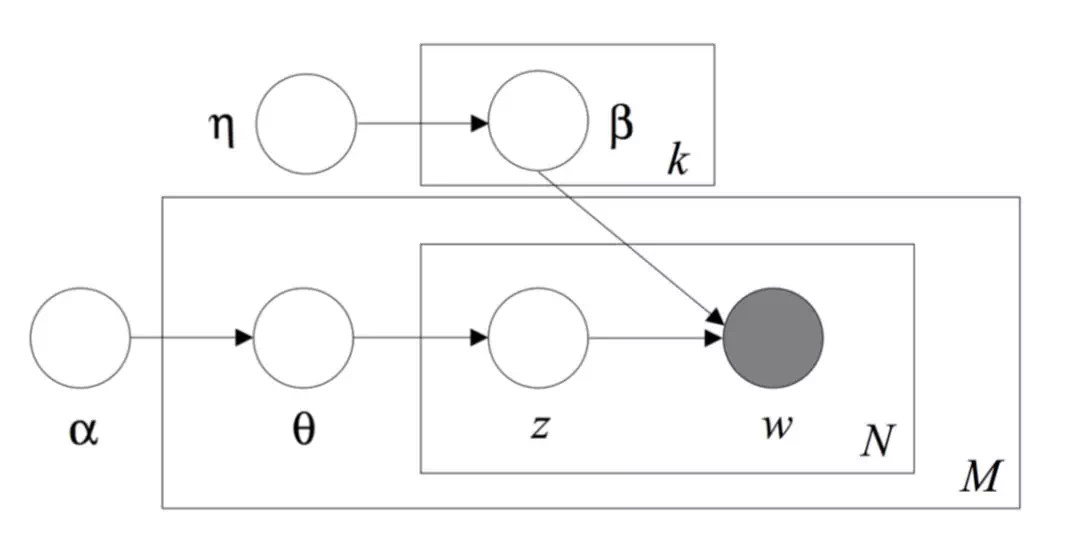
\includegraphics[width = \linewidth]{lda.png}
\caption{The caption of this figure.}
\label{fig:figure1label}
\end{figure}


In the LDA model, a document is generated as follows:
\begin{enumerate}
  \item Generate the  distribution of topic  by sampling from the Dirichlet distribution  with parameter $\alpha$ t;

  \item Sample the topic $z_{i,j}$ of $j$th word in the document $i$ by the ditribution given above;

  \item Sample the word distriution for each topic  and the distribution is subject to  Dirichlet distribution with parameter $\eta$;

  \item Finally sample the word  $w_{i,j}$from the multinomial distribution$\beta_{z_{i,j}}$.

\end{enumerate}

This probability graph can be decomposed into two parts:
\begin{enumerate}
  \item $$\alpha \rightarrow \theta  \rightarrow z $$
This process means that when generating the m-th document, a candidate for a topical toll is generated, and then the topic of each word in the document is randomly generated according to the toll;
  \item $$\eta \rightarrow \beta  \rightarrow w|k $$This process means that the word of the document can be  generated if the topic number is known. Firstly the word matrix will be gengerated by the Dirichlet distribution with the parameter $\eta$, and then the word distribution vector also will be selected when given the topic $k$. Finally the word is generated according to this vector;
\end{enumerate}

In the process of document construction,$ M$ documents correspond to $M$ independent Multinomial-Dirichlet conjugate structures, and $K$ topics also correspond to $K$ independent Multinomial-Dirichle conjugate structures. Among them, $M+K$ conjugate structures are all independent. Let’s discuss the document generative process further.


From the first decomposition\cite{coolaps},We know that $\alpha \rightarrow \theta$ represents the topic corresponding to all documents is subject to the Dirichlet distribution. Besides,  $\theta  \rightarrow z$  is to generate the topic corresponding to each word and the distribution of topic is subject to the multinomial distribution and the Dirichlet distribution is the conjugate distribution of the multinomial distribution. As a result, all the whole is a conjugate structure:
\begin{eqnarray*}
  f(z_k|\alpha) &=& \int f(z_k|p)f(p|\alpha) d_p \\
              &=& \int \prod_{k=1}^K p_k^{n_k} Dir(p|\alphha) d_p \\
              &=& \int \prod_{k=1}^K p_k^{n_k} \frac{1}{B(\alpha)}\prod_{k=1}^{K}p_k^{\alpha_k-1} d_p \\
              &=& \frac{1}{B(\alpha)}\int \prod_{k=1}{V}p_k^{n_k+\alpha_k-1} d_p \\
              &=& \frac{B(n_k+\alpha_k)}{B(\alpha)}
\end{eqnarray*}
Vector $n = (n_1,_2,..n_K)$ represents the number of words of topic $V$ in each document.
$B$ is the gamma function:
\[
  B(\alpha) = \frac{\prod_{i=1}^V\Gamma(\alpha_i)}{\Gamma(\sum_{i=1}^V \alpha_i)}
\]

For the second decomposition,We know that $\eta \rightarrow \beta$ represents the word-distribution corresponding to all topics, which is subject to the Dirichlet distribution. The process $\beta  \rightarrow w|k $  is to generate the word corresponding to each topic and it is subject to the multinomial distribution. Besides, the Dirichlet distribution is the conjugate distribution of the multinomial distribution. So that the second decoposition is also a conjugate structure:
\begin{eqnarray*}
  f(w|\beta) &=& \int f(w|\beta)f(\beta|\eta) d_{\beta} \\
              &=& \int \prod_{k=1}^V p_k^{n_k} Dir(p|\alpha) d_p \\
              &=& \int \prod_{k=1}^Vp_k^{n_k} \frac{1}{B(\alpha)}\prod_{k=1}^{V}p_k^{\alpha_k-1} d_p \\
              &=& \frac{1}{B(\alpha)}\int \prowd_{k=1}{V}p_k^{n_k+\alpha_k-1} d_p \\
              &=& \frac{B(n_k+\alpha_k)}{B(\alpha)}
\end{eqnarray*}
Vector $n = (n_1,_2,..n_V)$ represents the number of words generated by each topic $V$.

We assume two vector:
\[
  \vec{w} = (\vec{w_1},\vec{w_2},..\vec{w_k})
\]
\[
  \vec{z} = (\vec{z_1},\vec{z_2},..\vec{z_k})
\]


\begin{eqnarray*}
  p(\vec{w}\vec{z}|\alpha,\beta) & = & p(\vec{w}|\vec{z},\beta)p(\vev{z}|\alpha) \\
                                 & = & \prod_i^{K}\frac{B(\beta+n_k)}{\beta}\prod_i^M\frac{n_m+\alpha}{\alpha}
\end{eqnarray*}
$w_k$ indicates that these words were generated by the $k$th topic.

\subsection{Gibbs Sampling for LDA}
By the joint probability distribution $p(\vec{w},\vec{z}|\alpha,\beta)$ in the previous subsection, we can use Gibbs Sampling to approximate the distribution of topic and word. The $i$th word in the corpus  is denoted as $z_{i}$, where $i=(m,n)$ is a two-dimensional subscript, which corresponds to the $n$th word in the $m$ th document. According to the Gibbs Sampling algorithm in the second subsection, the conditional distribution corresponding to any coordinate axis are needed. Assuming the observed word $w_i=t$ and then by Bayes' rule, it is easy to get:
\begin{eqnarray*}
  p(z_i=k|\vec{z_{\neg_i}},\vec{w}) & \propto & p(z_i=k,w_i = t|\vec{z_{\neg_i}},\vec{w_{\neg_i}}) \\
  &=& \int p(z_i = k,w_i=t,\theta,\alpha|\vec{z_{\neg_i}},\vec{w_{\neg_i}})d_{\theta} d_{\alpha} \\
  &=& \int p(z_i=k,\theta|\vec{z_{\neg_i}},\vec{w_{\neg_i}}) p(w_i=t,\alpha|\vec{z_{\neg_i}},\vec{w_{\neg_i}})d_{\theta} d_{\alpha}\\

\end{eqnarray*}

Finally, we get the Gibbs Sampling formula of the LDA model as:
\[
p(z_i=k|\vec{z_{\neg_i}},\vec{w}) \propto \frac{n_{m,\neg{i}}^{(k)}+\alpha_k}{\sum^K (n_{m,\neg{i})}+\alpha_k)} *
 \frac{n_{k,\neg{i}}^{(t)}+\beta_t}{\sum^V (n_{m,\neg{i})}+\beta_t)}
\]


The equation on the right can be seen as \[
  p(topic|doc)*p(word|topic)
\]


The LDA Gibbs sampling algorithm can be summarized as follow. The first is the training process:
\begin{enumerate}
  \item  Choose the  number of topics $k$ and the proper hyperparameter vector $\vec{\alpha}$ and $\vec{\beta}$;
 \item Randomly assign a topic number $z$ for every word in each document;
 \item Rescan the corpus, for each word, use Gibbs sampling formula to update its topic;
  \item Repeat the Gibbs sampling based on coordinate axis rotation in step 3 until the Gibbs sampling converges.
  \item Count the topic of each word in each document in the corpus and then get the document topic distribution $\theta_d$, which is enable to iference the topic of each document. Besides,word distribution $\beta_k$ also will be saved.
\end{enumerate}

With the LDA model, for the new document doc, the topic-word matrix is stable and is provided by the model obtained from the training corpus, so we only topic distribution of the document need to be estimated. The specific algorithm is as follows:
\begin{enumerate}
  \item  For each word $w_i$ in the current document, randomly initialize a topic number $z$.
  \item Use Gibbs Sampling formula to resample the topic of each word $w_i$.
  \item  Repeat the above process until Gibbs Sampling convergence.
  \item Statistics on the topic distribution in the document, the distribution is $\theta_i$.
\end{enumerate}

\subsection{Perplexity and Inference}

In information theory, perplexity\cite{per} is a measure of judging the probability model or probability distribution prediction, and can be used to evaluate thetopic model.
\[
  perplexity(D) = exp(-\frac{\sum_{k=1}^{M}p(\vec{w_k})}{\sum_{k=1}^{M}N_k})
\]
The denominator is the sum of all the words in the test set, that is, the total length of the test set. Where $p(\vec{w_k})$ refers to the probability of each word of document $k$ in the test set.
\begin{eqnarray*}
  p(\vec{w_k}) &=&\prod_{i=1}^{V}p(w_k^{(i)})\\
               &=&\prod_{i=1}^{V}\int p(w_k^{(i)}|z_i)p(z_i)d_{z_i}
\end{eqnarray*}
